% !TeX spellcheck = en_US
\subsection{Hybrid encoding integrating Log and Order encoding}
With the idea of exploiting the pros of each encoding and avoid their cons a new hybrid encoding emerged. Log encoding represents each value in CSP's domain as binary integer and as a result generates small SAT problems regarding the number of propositional variables and the number of constraints (compared to the direct encoding since no additional clauses are required). On the other hand, the order encoding is known for its performance, then it generates additional variables that bounds the SAT problem and make it more liable for being solved directly by the one literal rule using unit propagation instead of branching. But each encoding has its limitations; for instance: the order encoding generate huge SAT instances when the CSP domain or the arity of the constraints becomes large. Likewise, the log encoding suffers from poor performance in general.

\subsubsection{Core idea}
Other encodings have already proposed merging multiple encodings together to benefit from each of them, but no true hybridization have been applied. Each variable was encoded with both types of used encodings and then additional clauses were added to channel both types of generated constraints together. This proposed encoding works without channeling the constraints and using a criterion to determinate the appropriate encoding for each variable. Therefore, the resulted constraints can contain both types of encoded variables and don't require additional constrains channeling. Log and order encodings operates as partial encoding, while their use is controlled by the criterion. The authors proposed the domain product as the classification criterion but other criteria could have been used. \cite{soh2015hybrid}

\subsubsection{Performance test}
The authors implemented their own CSP-Solver and tested it against two sets of benchmark problems. The first set was handmade and the second one was selected from a CSP solver competition. In both tests the hybrid encoding showed better results and superior performance compared to applying the partial encodings alone. Detailed tables with exact figures and details about the test environment are provided in the original paper \cite{soh2015hybrid}. It should be noted that this some problems with high artiy and domain size could be only solved with the hybrid encoding in a reasonable amount of time.

The following Venn diagram in Fig.\ref{fig:hybrid_encoding_venn} shows the number of instances from the second benchmark set solved by each encoding. Clearly the hybrid encoding with 815 solved instances dominates both log and direct encoding. Only 6 problems were unsolvable by the new hybrid encoding, which is the smallest number among the other encodings. The paper \cite{soh2015hybrid} also compares the 3 encodings regarding the average CPU time needed for solving the first benchmark set. As expected, the hybrid encoding correctly inherits the advantages of both encodings and comes out as the clear winner.

\begin{figure}[H]
	\centering

	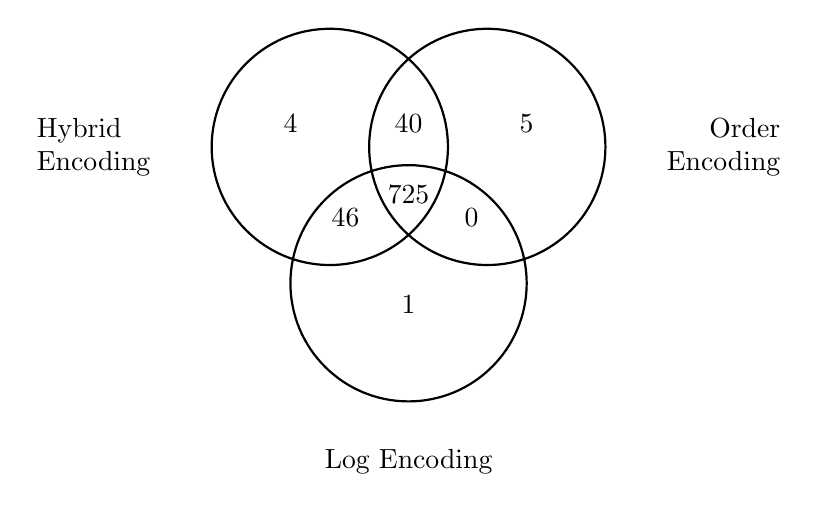
\begin{tikzpicture}[thick]
		 % Draw the circles
		 \draw (0,0) circle (1.5cm);
		 \draw (-60:2cm) circle (1.5cm);
		 \draw (0:2cm) circle (1.5cm);
		 
		 % Label the circles
		 \draw[align=left] (-3,-0) node {Hybrid\\Encoding};
		 \draw (1,-4) node {Log Encoding};
		 \draw[align=right] (5,0) node {Order\\Encoding};
		 \draw (-0.5,0.3) node {4};
		 \draw (1,0.3) node {40};
		 \draw (2.5,0.3) node {5};
		 \draw (0.2,-0.9) node {46};
		 \draw (1,-0.6) node {725};
		 \draw (1.8,-0.9) node {0};
		 \draw (1,-2) node {1};
	\end{tikzpicture}
	
	\captionsetup{justification=centering,margin=2cm}
	\caption{Number of solved instances from the benchmark set by each encoding}
	\label{fig:hybrid_encoding_venn}
\end{figure}
